%Capítulo 2 - Fundamentos de pompressão de imagens e vídeos%

\thispagestyle{fancy}

Neste capítulo abordam-se aspectos teóricos do processo de compressão de imagens e vídeos. Primeiramente, o conceito de redundância, presente em \textit{arrays} 2D, será abordado, fazendo-se a relação com a teoria da 
informação. Em seguida, é discutida uma possível classificação dos tipos de compressão com base na preservação do sinal original. Por fim, analisa-se o funcionamento dos padrões JPEG e MPEG-1.

\section{Redundância}
\label{redundancia}

O processo de compressão de dados consiste em reduzir a quantidade de bits necessária para representar uma determinada informação. Neste 
contexto, os conceitos de dados e informação são diferentes, pois os dados são os meios pelos quais as informações são transmitidas 
\cite{Gonzalez2006}.

Seguindo esta linha de raciocínio, uma informação pode ser representada de infinitas maneiras. Assim sendo, o questionamento a ser respondido quando se objetiva a compressão de dados é: qual representação forneceria o menor volume de dados sem que houvesse perda de informação?

A compressão é obtida através da eliminação dos dados redundantes presentes na representação de uma informação mantendo um dado critério de fidelidade. Em se tratando de 
\textit{arrays} bidimensionais, os principais tipos de redundância são \cite{Gonzalez2006}:

\begin{itemize}
 \item \textit{Redundância de codificação}: ocorre quando a quantidade de bits utilizada para representar os símbolos de uma determinada informação é superior à quantidade necessária. Este tipo de redundância é muito comum em métodos de codificação que trabalham com a atribuição de palavras-código de tamanho fixo.
 
 \item \textit{Redundância espacial e temporal}: devido à grande parte dos \textit{pixels} presentes em um \textit{array} 2D estarem espacialmente
 correlacionados, surge a redundância espacial. Já as sequências de vídeo estão sujeitas a mais outro tipo de redundância, a temporal, em que os pixels de quadros vizinhos encontram-se correlacionados devido à grande semelhança entre eles. Isso significa dizer que é possível alcançar maiores
taxas de compressao em vıdeos, do que em imagens estáticas.
 
 \item \textit{Redundância psicovisual}: é originada a partir das características do sistema visual humano. Sua resposta aos estímulos visuais é uma função
 não linear de grandezas físicas, como intensidade luminosa e cores. Neste contexto, pesquisas a respeito do funcionamento e comportamento do sistema visual humano são de grande importância para que possam ser gerados modelos matemáticos que representem características de tal sistema.
\end{itemize}



A quantificação do volume de dados redundantes presente em uma representação de imagem é necessária para que se possa avaliar a compressão obtida. Sendo assim, assumindo que $ b $ e $ b' $ são, respectivamente, o volume de dados presentes na representação real de uma imagem e o volume de dados
presentes em uma representação comprimida da mesma, a \textit{redundância relativa} $ R $ é dada por \cite{Gonzalez2006}
\begin{equation}
\label{eqR}
 R = 1-\frac{1}{c}
\end{equation}
em que $c$ é a \textit{taxa de compressão}, definida como sendo
\begin{equation}
\label{eqc}
 c=\frac{b}{b'}
\end{equation}

\section{Teoria da Informação}
\label{teoriadainformacao}

Durante a década de $ 40 $, no período da Segunda Guerra Mundial, o processo de troca de informações tornou-se fundamental. Dessa forma, surgiu a necessidade de estabelecer um limite mínimo de volume de bits necessário para a transmissão de uma determinada informação, a fim de otimizar a utilização do canal disponível.

Neste contexto, Claude Elwood Shannon ficou conhecido com o ``pai da teoria da informação'' ao propor com sucesso uma maneira de medir a incerteza sobre espaços desordenados \cite{shannon48}.

\subsection{Primeiro teorema de Shannon}
\label{shannonTheorem}
Através do teorema da codificação sem perda \cite{shannon48} pode-se provar que é possível representar a saída de um sistema sem memória com uma média $ H $ de unidades de informação por pixel,
\begin{equation}
\label{eqshannonTheorem}
\lim_{n \to \infty}
\left[\frac{L_{avg,n}}{n} \right]= H
\end{equation}
em que, $ L_{avg,n} $ é o número médio de códigos símbolo necessários para representar todos os grupos de $ n $ símbolos e $ H $ é a entropia.

\subsection{Entropia}
\label{entropia}

A entropia, equação \ref{eqentropia}, é uma medida utilizada em diversas áreas do conhecimento, como na química e física. Em se tratando de informações, a entropia representa o grau de incerteza de uma fonte.

Sendo (\textit{$a_{1}$,$a_{2}$,...,$a_{J}$}) o conjunto de símbolos (eventos) emitidos por uma determinanda fonte e $P(a_{1}), P(a_{2}), ..., P(a_{j})$ suas respectivas probabilidades de ocorrência, a informação contida em cada símbolo é
\begin{equation}
\label{eqentropia}
I(a_i) = \log_b{\frac{1}{P(a_{i})}}
\end{equation}
e a entropia é dada pela informação média dos símbolos.

\begin{equation}
\label{eqentropia}
H = -\sum_{j=1}^J P(a_{j})\log_b{P(a_{j})}
\end{equation}

No caso de imagens digitais, em que a unidade de representação é o \textit{bit}, tem-se que $ b = 2$ na equação \ref{eqentropia}.

\section{Métodos básicos de compressão}
\label{metodosdecompressao}

De maneira geral, existem dois tipos de compressão, com e sem perda, com as seguintes carcterísticas:

\begin{itemize}
\item Sem perda: objetiva comprimir o volume de dados necessários para representar uma dada informação sem que a mesma seja afetada. Para isso, códigos diferentes do código natural são atribuídos aos símbolos, a fim de reduzir a redundância de codificação. 

\item Com perda: objetiva alcançar um maior nível de compressão através da eliminação de elementos com base em critérios de qualidade exigidos pela aplicação de interesse.
\end{itemize}

\subsection{Métodos}
\label{metodos}

Existem vários métodos de codificação com e sem perda. Dentre eles, os mais utilizados são:

\begin{enumerate}
\item Sem perda:
\begin{itemize}
\item Huffman: a codificação de Huffman \cite{huf52} é um método de codificação de tamanho variável que consiste na atribuição de palavras código menores para símbolos mais frequentes e maiores para os símbolos menos frequentes.

O primeiro passo é rearranjar as probabilidades dos símbolos da fonte em ordem decrescente e fazer reduções sucessivas agrupando os símbolos de menor probabilidade de ocorrência, como na figura \ref{fig:huff_red}.

\begin{figure}[!ht]

\begin{minipage}{\textwidth}
    \begin{minipage}{.4\textwidth}
      \centering
      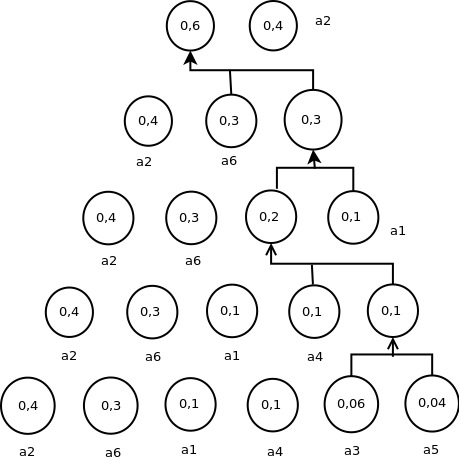
\includegraphics[width=.79\textwidth]{./Figures/png/huff_red.png}
      \caption{Reduções da fonte \cite{Gonzalez2006}.}
      \label{fig:huff_red}
    \end{minipage}
    \begin{minipage}{.56\textwidth}
    \center
      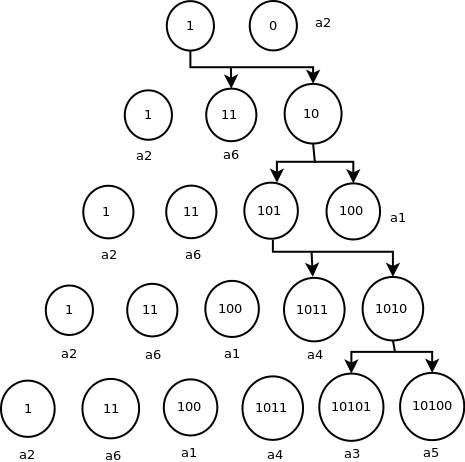
\includegraphics[width=.56\textwidth]{./Figures/png/huff_cod.png}
      \caption{Codificação da fonte reduzida \cite{Gonzalez2006}.}
      \label{fig:huff_cod}
    \end{minipage}
  \end{minipage}
\end{figure}

Por fim, deve-se codificar cada fonte reduzida seguindo o sentido inverso das reduções atribuindo $ 0 $ para as menores probabilidades e $ 1 $ para as maiores, ou vice-versa, como na figura \ref{fig:huff_cod}. Desta forma cada símbolo terá uma única palavra código cujo tamanho é inversamente proporcional a sua probabilidade de ocorrência.

\item Codificação aritmética: é um método de codificação de tamanho variável que trabalha de maneira bem diferente em relação à codificação de Huffman. Sua abordagem atribui faixas de valores, entre $ 0 $ e $ 1 $, para cada símbolo e por fim atribui palavras código aos intervalos \cite{Bhaskaran:1997:IVC:549617}.

Considerando o alfabeto $ s = (s1,s2,s3,s4) $, suponhamos que se queira codificar a mensagem $ s1s2s4$. Primeiramente calculam-se as probabilidades dos símbolos-fonte, as quais irão ocupar seguimentos proporcionais do intervalo $[0, 1]$. Depois deve-se fazer sucessivas divisões proporcionais dos símbolos dentro dos seguimentos, seguindo a ordem dos símbolos da mensagem, como na tabela \ref{arit_cod}.

\begin{table}[!ht]
\centering
\begin{tabular}{|c|c|c|c|c|c|}
\hline
$ s $ & $ p(s) $ & Faixa & $ s1$ & $ s1s2 $             & $ s1s2s4 $             \\ \hline 
s1            & 0,2           & {[}0,0; 0,2)         & {[}0,0; 0,04)  & {[}0,04;  0,048) & {[}0,072; 0,0736)   \\ \hline
s2            & 0,2           & {[}0,2; 0,4)         & {[}0,04; 0,08) & {[}0,048; 0,056) & {[}0,0736; 0,0752) \\ \hline
s3            & 0,4           & {[}0,4; 0,8)         & {[}0,08; 0,16) & {[}0,056; 0,072) & {[}0,0752; 0,0784) \\ \hline
s4            & 0,2           & {[}0,8; 1,0)         & {[}0,16; 0,2)  & {[}0,072; 0,08)  & {[}0,0784; 0,08)    \\ \hline
\end{tabular}
\caption{Exemplo de codificação aritmética.}
\label{arit_cod}
\end{table}

Por fim, escolhe-se um número dentro do intervalo atribuído para uma determinada mensagem que deverá representá-la	. No caso da mensagem $ s1s2s4 $,  foi atribuída a faixa $ [0,072; 0,08) $ e cada valor dentro da mesma poderá ser escolhido para representar esta mensagem.

\item Run-length: inicialmente produzida para a compressão para ser utilizada na tecnologia de FAX, cujas imagens são binárias. 

A codificação run-length é executada linha a linha começando com o valor inicial ($ 0 $ ou $ 1 $) seguido pelo número de repetições sucessivas. Quando houver a mudança de valor basta acrescentar o números de repetições sucessivas, pois sabe-se que o próximo valor é a negação do anterior.

\end{itemize}
\item Com perda:
\begin{itemize}
\item DPCM: Considerando que uma determinada amostra pode ser representada por 

\begin{equation}
\label{sinal_orig}
f(n) = \hat{f}(n) + e(n)
\end{equation}

em que $ \hat{f}(n) $ é uma aproximação da amostra original e $ e(n) $ é erro associado à mesma, o erro médio quadrático entre $ f $ e $ \hat{f} $  pode ser minimizado através de uma melhor aproximação do sinal original. 

Na codificação DPCM (Differential Pulse-Code Modulation), se $ e(n) \rightarrow 0 $, temos que a aproximação do sinal original pode ser representada por uma combinação linear descrita por

\begin{equation}
\label{sinal_pred}
\hat{f}(n) = \sum_{\substack{i=1}}^{m}\alpha_{i}f(n-i)
\end{equation}

em que os coeficientes são calculados através da minimização da expressão \ref{minimization}.

\begin{equation}
\label{minimization}
E \{ e(n)^{2} \} = E\left\{ \left[ f(n)- \sum_{\substack{i=1}}^{m}\alpha_{i}f(n-i)\right] ^{2} \right\}
\end{equation}

\item Codificação baseada em transformada de blocos: é uma técnica de compressão que consiste em dividir uma imagem em blocos não sobrepostos de tamanhos iguais (geralemente $ 8 \times 8 $). Uma transformada linear reversível, como a transformada de Fourier e a transformada cosseno, é utilizada para mapear estes blocos no domínio da frequência que por fim serão submetidos a um processo de quantização \cite{Gonzalez2006}.
\end{itemize}
\end{enumerate}

\section{Os padrões JPEG e MPEG-1}
\label{JPEGeMPEG}

O processo evolutivo da espécie humana deu-se de forma que a visão foi o sentido que mais se desenvolveu: cerca de $ 80-90\% $ dos neurônios estão relacionados com o processamento de informações visuais \cite{Young1991}. Dessa forma, não é de se surpreender que imagens e vídeos sejam cada vez mais explorados digitalmente.

Seguindo essa tendência, intensificaram-se as buscas por métodos capazes de otimizar a utilização da banda de transmissão sem que a informação seja prejudicada. Com base nisso surgiu a necessidade de padronização de métodos de compressão de imagens e vídeos, dando origem ao JPEG \cite{international1993ccitt}  e MPEG-1 \cite{telecommunication1993itu}, \cite{Bialkowski:2007:FVT:1290871.1290876}, \cite{1218189}.

\subsection{JPEG}
\label{jpeg}

Em meados da década de $ 80 $, a União Internacional de Telecomunicações (ITU, do inglês Iternational Telecommunication Union) concentrou seus esforços para a criação de um padrão de compressão de imagens estáticas. Desta forma deu-se a origem do JPEG.

Este padrão consiste em uma combinação de duas técnicas de compressão, com e sem perda (quantização e codificação de entropia). Como pode ser notado nas figuras \ref{fig:jpeg_enc} e \ref{fig:jpeg_dec}, o codificador e o decodificador, respectivamente, do \textit{JPEG baseline} \cite{Gonzalez2006} são destacados pela cor azul.

\begin{figure}[!ht]
  \begin{center}
    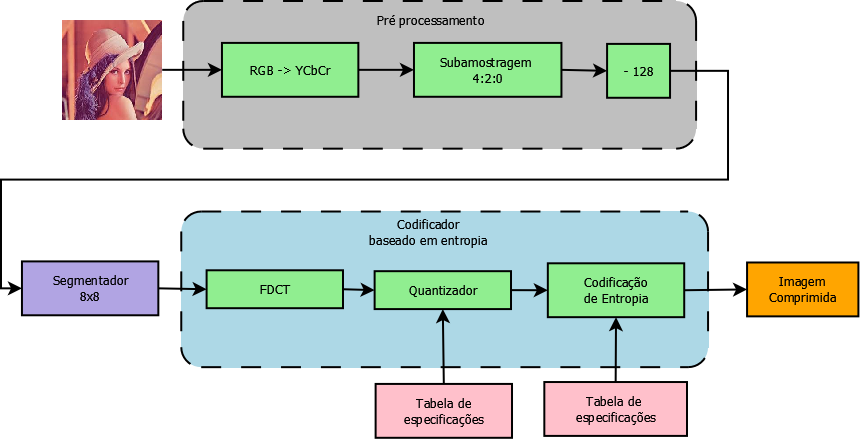
\includegraphics[scale=0.35]{./Figures/png/jpeg_encoder.png}
      \caption{Diagrama de blocos do codificador JPEG.}
      \label{fig:jpeg_enc}
  \end{center}
\end{figure}

\begin{figure}[!ht]
  \begin{center}
    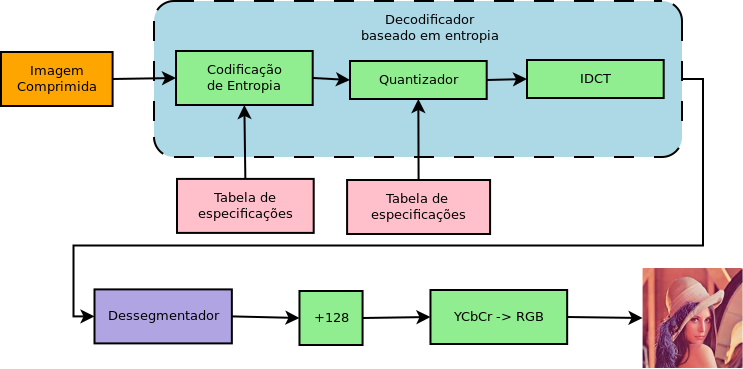
\includegraphics[scale=0.45]{./Figures/png/jpeg_decoder.png}
      \caption{Diagrama de blocos do decodificador JPEG.}
      \label{fig:jpeg_dec}
  \end{center}
\end{figure}

\subsubsection{JPEG baseline}
\label{JPEG_baseline}

Antes de detalhar o JPEG \textit{baseline} é importante citar que os canais de imagens RGB possuem um alto grau de correlação e carregam grande quantidade de informações espaciais, impossibilitando a eliminação de componentes da informação sem que a mesma seja fortemente afetada. Por isso o padrão JPEG trabalha com imagens YCbCr, que concentram a maior parte das informações espaciais no canal da luminância (Y) e as informações de cores nos canais restantes (Cb e Cr), possibilitando a eliminação de componentes de informação através da subamostragem da crominância \cite{Bhaskaran:1997:IVC:549617} no formato 4:2:0, detalhado no apêncide \ref{cro_diz}.

No sistema \textit{baseline} \cite{Gonzalez2006} o processo de compressão é composto por quatro passos sequenciais: segmentação, cálculo da transformada cosseno discreta, quantização e determinação dos códigos de tamanho variável para cada símbolo.

Inicialmente, a imagem é subdividida em blocos 8 $\times$ 8. Depois que os blocos são encontrados, seus valores são deslocados, subtraindo $ 2^{k-1} $ unidades, em que $ 2^{k} $ é o número máximo de níveis de intensidade. Então, aplica-se a transformada cosseno, onde $ p(x,y) $ é o valor do pixel na posição $ (x,y) $ e $ N $ é a ordem do bloco (oitava ordem) \cite{cabeen1998image},
\begin{equation}
\label{dct_eq}
D(i,j) = \frac{1}{\sqrt{2N}} C(i)C(j) \sum\limits_{x=0}^{N-1} \sum\limits_{y=0}^{N-1} p(x,y) \cos \left[ \frac{(2x+1)i \pi}{2N} \right] \cos \left[ \frac{(2y+1)j \pi}{2N} \right]
\end{equation}
\begin{equation}
C(u) = \begin{cases}
\frac{1}{\sqrt{2}} \quad \textrm{se } u = 0 \\
1 \quad \textrm{se } u > 0 \\ 
\end{cases} 
\end{equation}
 seguida pelo processo de quantização,
\begin{equation}
\label{eq_quant}
\hat{T}(u,v) = round \left(\frac{T(u,v)}{Z(u,v)}\right)
\end{equation}
em que $ \hat{T}(u,v) $ é o bloco quantizado (Fig.\ref{subimage_quant}), $ T(u,v) $ é o bloco transformado e $ Z(u,v) $ é a tabela de quantização padrão (Fig.\ref{quant_standard}) multiplicada por um fator de qualidade.

Através de experimentos subjetivos a respeito da percepção visual humana obteve-se a tabela de quantização padrão do JPEG. A utilização da mesma gera uma qualidade visual de $ 50\% $, que pode ser alterada multiplicando-a por um fator de qualidade: se a qualidade desejada for superior a $ 50 \% $ o fator usado deve ser $ (100-qualidade)/50 $, caso contrário o fator é $ 50/qualidade $.

\begin{figure}[!ht]\label{figuras_jpeg}
\subfigure[]{\label{quant_standard}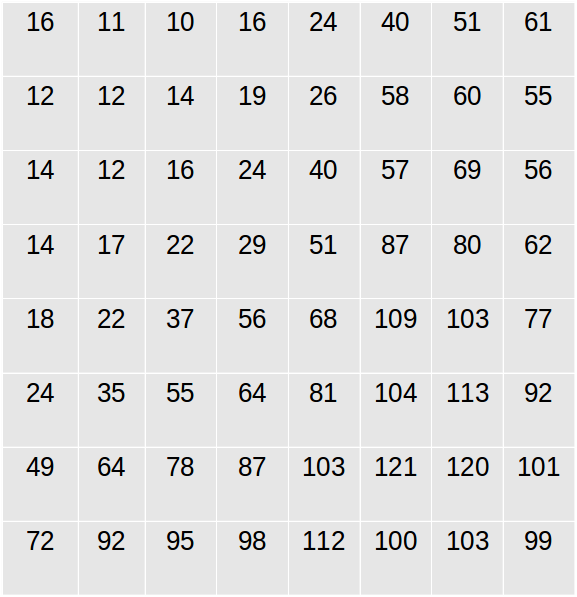
\includegraphics[width=.5\textwidth, height=.5\textwidth]{./Figures/png/tabela_padrao.png}}
\subfigure[]{\label{zigzag}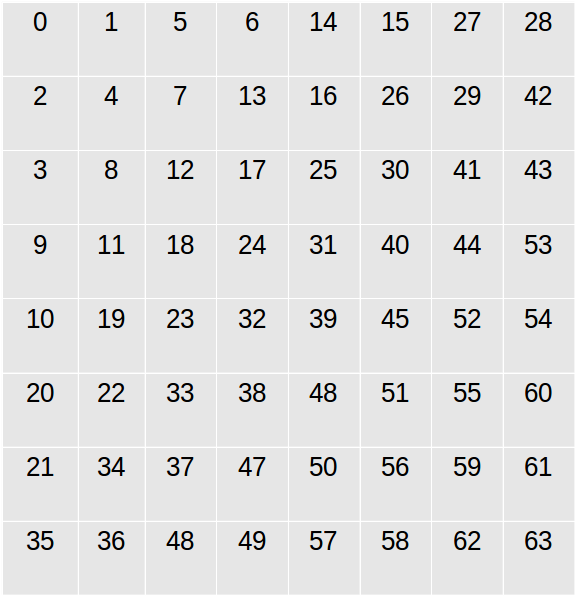
\includegraphics[width=.5\textwidth, height=.5\textwidth]{./Figures/png/zigzag.png}}
\subfigure[]{\label{subimage}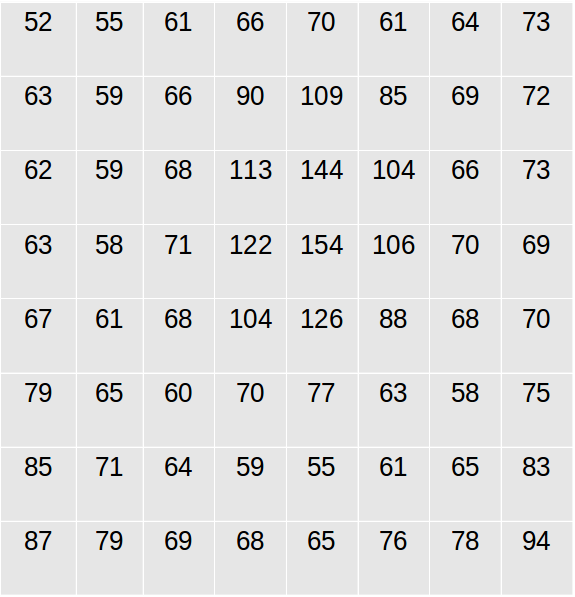
\includegraphics[width=.5\textwidth, height=.5\textwidth]{./Figures/png/subimage.png}}
\subfigure[]{\label{subimage_quant}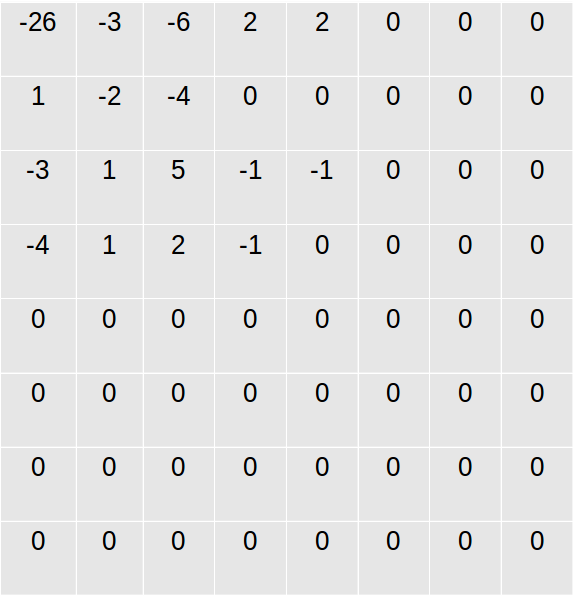
\includegraphics[width=.5\textwidth, height=.5\textwidth]{./Figures/png/subimage_quant.png}}
\caption{(a): Tabela de quantização padrão ($ 50 \% $); (b): Padrão zigzag; (c): Exemplo de subimagem; (d): Subimagem quantizada.}
\label{comp_visual}
\end{figure}

%\begin{table}[!ht]
%\begin{minipage}{.5\textwidth}
%\centering
%\begin{tabular}{|c|c|c|c|c|c|c|c|}
%\hline
%16 & 11 & 10 & 16 & 24  & 40  & 51  & 61  \\ \hline
%12 & 12 & 14 & 19 & 26  & 58  & 60  & 55  \\ \hline
%14 & 13 & 16 & 24 & 40  & 57  & 69  & 56  \\ \hline
%14 & 17 & 22 & 29 & 51  & 87  & 80  & 62  \\ \hline
%18 & 22 & 37 & 56 & 68  & 109 & 103 & 77  \\ \hline
%24 & 35 & 55 & 64 & 81  & 104 & 113 & 92  \\ \hline
%49 & 64 & 78 & 87 & 103 & 121 & 120 & 101 \\ \hline
%72 & 92 & 95 & 98 & 112 & 100 & 103 & 99  \\ \hline
%\end{tabular}
%\caption{Tabela de quantização padrão ($ 50 \% $).}
%\label{standard_table}
%\end{minipage} 
%\begin{minipage}{.5\textwidth}
%\centering
%\begin{tabular}{|c|c|c|c|c|c|c|c|}
%\hline
%0  & 1  & 5  & 6  & 14 & 15 & 27 & 28 \\ \hline
%2  & 4  & 7  & 13 & 16 & 26 & 29 & 42 \\ \hline
%3  & 8  & 12 & 17 & 25 & 30 & 41 & 43 \\ \hline
%9  & 11 & 18 & 24 & 31 & 40 & 44 & 53 \\ \hline
%10 & 19 & 23 & 32 & 39 & 45 & 52 & 54 \\ \hline
%20 & 22 & 33 & 38 & 46 & 51 & 55 & 60 \\ \hline
%21 & 34 & 37 & 47 & 50 & 56 & 59 & 61 \\ \hline
%35 & 36 & 48 & 49 & 57 & 58 & 62 & 63 \\ \hline
%\end{tabular}
%\caption{Padrão zigzag.}
%\label{zigzag}  
%\end{minipage}% 
%\vfill
%\begin{minipage}{.5\textwidth}
%\centering
%\begin{tabular}{|c|c|c|c|c|c|c|c|}
%\hline
%52 & 55 & 61 & 66 & 70  & 61  & 64  & 73  \\ \hline
%63 & 59 & 66 & 90 & 109  & 85  & 69  & 72  \\ \hline
%62 & 59 & 68 & 113 & 144  & 104  & 66  & 73  \\ \hline
%63 & 58 & 71 & 122 & 154  & 106  & 70 & 69  \\ \hline
%67 & 61 & 68 & 104 & 126  & 88 & 68 & 70  \\ \hline
%79 & 65 & 60 & 70 & 77 & 63 & 58 & 75 \\ \hline
%85 & 71 & 64 & 59 & 55 & 61 & 65 & 83 \\ \hline
%87 & 79 & 69 & 68 & 65 & 76 & 78 & 94  \\ \hline
%\end{tabular}
%\caption{Exemplo de subimagem.}
%\label{subimage_example}
%\end{minipage} 
%\begin{minipage}{.5\textwidth}
%\centering
%\begin{tabular}{|c|c|c|c|c|c|c|c|}
%\hline
%-26 & -3 & -6 & 2  & 2  & 0 & 0 & 0 \\ \hline
%1   & -2 & -4 & 0  & 0  & 0 & 0 & 0 \\ \hline
%-3  & 1  & 5  & -1 & -1 & 0 & 0 & 0 \\ \hline
%-4  & 1  & 2  & -1 & 0  & 0 & 0 & 0 \\ \hline
%0   & 0  & 0  & 0  & 0  & 0 & 0 & 0 \\ \hline
%0   & 0  & 0  & 0  & 0  & 0 & 0 & 0 \\ \hline
%0   & 0  & 0  & 0  & 0  & 0 & 0 & 0 \\ \hline
%0   & 0  & 0  & 0  & 0  & 0 & 0 & 0 \\ \hline
%\end{tabular}
%\caption{Subimagem da tabela \ref{subimage_example} quantizada.}
%\label{subimage_quantized}  
%\end{minipage}
%\end{table}

Por fim, os coeficientes dos blocos quantizados são reordenados no padrão zigzag (Tabela \ref{zigzag}), resultando em um vetor,

\begin{minipage}{1.\textwidth}
\centering
[-26 -3 1 -3 -2 -6 2 -4 1 -4 1 1 5 0 2 0 0 -1 2 0 0 0 0 0 -1 -1 EOB]
\end{minipage}
e codificados com base nas tabelas de Huffman pré definidas, as quais agrupam derivações dos métodos DPCM e run-length\footnote{A palavra código EOB significa que os coeficientes são iguais a $ 0 $ daquele ponto até o último coeficiente AC.}, como descrito no Apêndice \ref{ap_JPEG}.

O processo de decodificação é obtido através da simples inversão da ordem das operações.

\subsection{MPEG-1}
\label{mpeg}

O padrão H.261 \cite{ITU.1993} é um método versátil de compressão de vídeos com perda, pois pode ser aplicado a uma grande variedade de formatos de entrada. Porém, foi otimizado para aplicações que suportam taxas contínuas de transferência de bits de $ 1,5 $ Mbps.

Como mencionado na Seção \ref{redundancia}, os  vídeos estão sujeitos à redundância temporal devido à alta semelhança entre imagens vizinhas. Por isso, antes de falar do MPEG-1, é conveniente abordar o processo de estimação e compensação de movimentos baseado em blocos, a fim de eliminar a redundância temporal.

\subsubsection{Estimação e compensação de movimentos baseados em blocos}
\label{Est_Comp_Mov}

Objetivando-se reduzir a redundância temporal entre imagens consecutivas poder-se-ia pensar em armazenar apenas a diferença entre duas imagens, porém este processo pode ser otimizado através da utilização de macroblocos. Por isso pode-se dizer que este método é uma variação da codificação DPCM.

Macroblocos são compostos por 4 blocos $ n\times n $, na maioria das vezes 8$ \times $8. Na Figura \ref{fig:macrobloco} é representado um macrobloco subamostrado no padrão 4:2:0. Este padrão trabalha da seguinte forma:

\begin{figure}[!ht]
\begin{center}
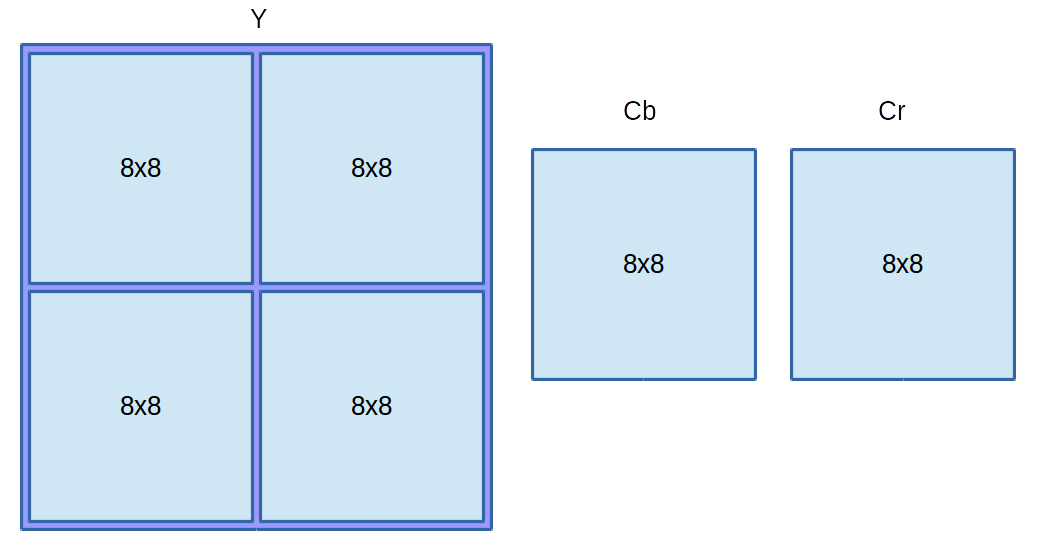
\includegraphics[scale=0.4]{./Figures/png/macrobloco.png}
\caption{Macrobloco dizimado no padrão 4:2:0.}
\label{fig:macrobloco}
\end{center}
\end{figure}

Utilizando macroblocos para a encontrar a diferença entre imagens consecutivas torna-se possível a minimização do erro médio absoluto (MAE, do inglês \textit{mean absolute error}) 
\begin{equation}
MAE(i,j) = \frac{1}{MN} \sum_{k=0}^{M-1} \sum_{l=0}^{N-1} |C(x+k,y+l)-R(x+i+k,y+j+l)
\end{equation}
da mesma, em que $C$ é um macrobloco da imagem de atual e $R$ o possível macrobloco correspondente na imagem de referência.

Inicialmente se considera uma imagem atual, em que se tem um macrobloco de dimensões 16$ \times $16 e uma imagem anterior com um macrobloco de mesmas dimensões com a menor diferença possível. Estes dois macroblocos possuem um deslocamento relativo designado por ``vetor de deslocamento'' e esta diferença é designada por ``erro de predição''. A este processo dá-se o nome de compensação de movimento para frente (Fig. \ref{fig:foreward_prediction}).

\begin{figure}[!ht]
\begin{center}
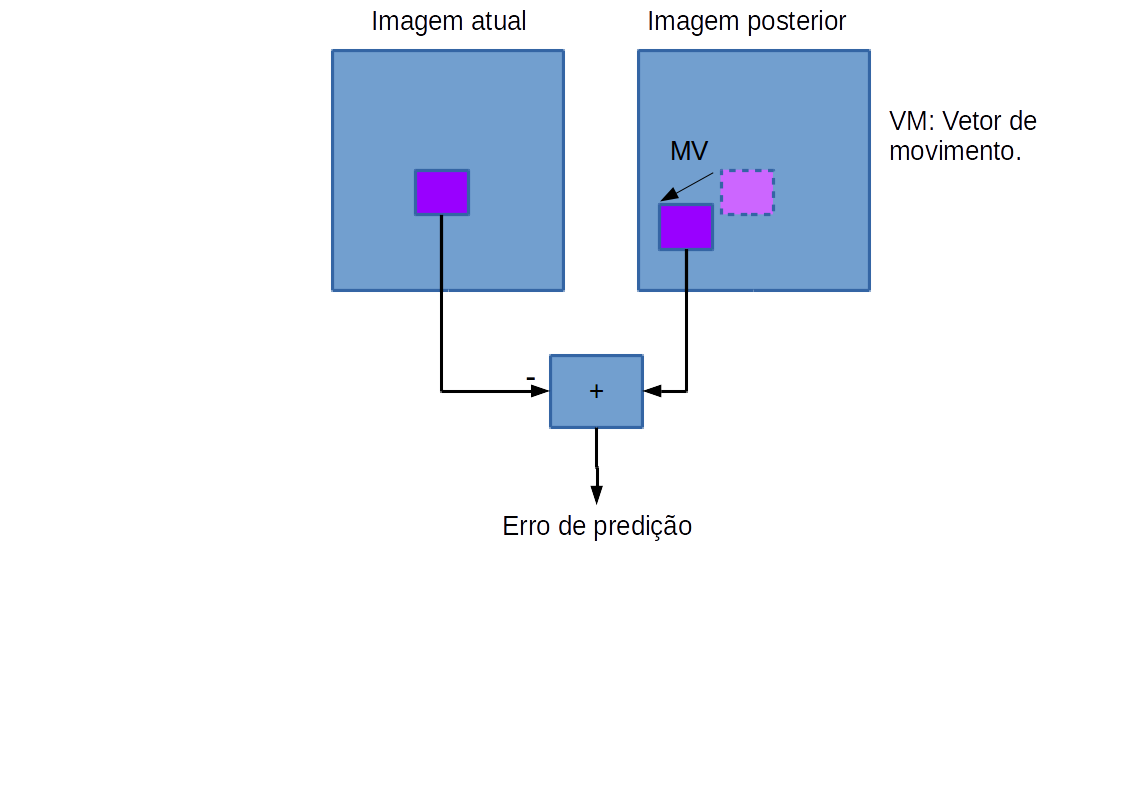
\includegraphics[scale=0.5]{./Figures/png/foreward_prediction.png}
\caption{Compensação de movimento pra frente.}
\label{fig:foreward_prediction}
\end{center}
\end{figure}

Também pode-se estender este raciocíno, tomando como base uma imagem atual, uma anterior e uma posterior a fim de obter a menor diferença possível. Este processo chama-se compensação de movimento bidirecional (Fig. \ref{fig:bidirectional_prediction}).

\begin{figure}[!ht]
\begin{center}
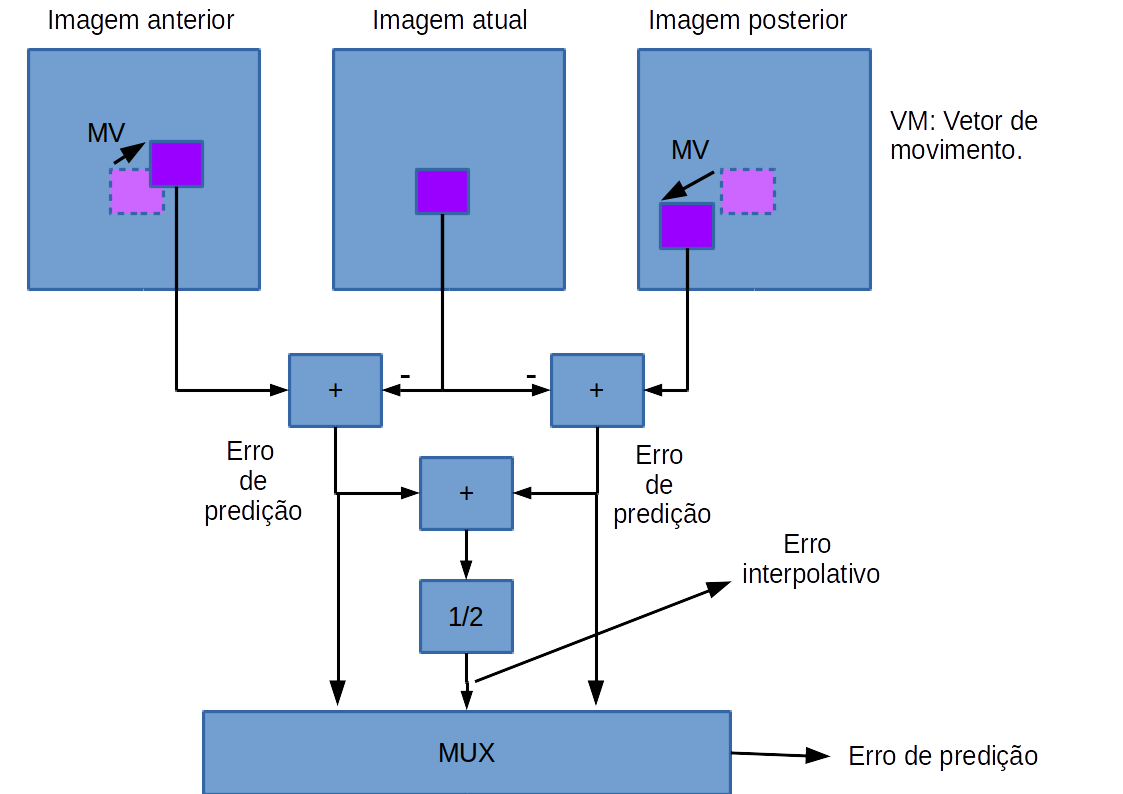
\includegraphics[scale=0.5]{./Figures/png/bidirectional_prediction.png}
\caption{Compensação de movimento bidirecional.}
\label{fig:bidirectional_prediction}
\end{center}
\end{figure}

A diferença fundamental entre os dois modelos de compensação de movimento é que o bidirecional trabalha com três erros de predição (para trás, para frente ou interpolativo) e não um, como na predição para frente. 

\subsubsection{Métodos de busca}

Há muitas formas de estimar os vetores de deslocamento dos macroblocos, algumas possibilitam uma maior precisão ao encontrar o melhor candidato, outras possibilitam uma maior velocidade na determinação do mesmo.

Dentre os métodos básicos, pode-se citar \cite{Bhaskaran:1997:IVC:549617}:
\begin{enumerate}
\item {\bf Busca completa:} é o método mais simples e garante que o melhor candidato seja encontrado, obtendo o menor valor possível do MAE.

Consiste na definição de uma área de busca de $ p $ pixels para os lados, para cima e para baixo a partir do canto superior esquerdo do macrobloco. Para cada um dos $ (2p+1)^2 $ pixels da área de busca serão formados os possíveis macroblocos a serem submetidos ao critério de minimização do MAE.

\item {\bf Busca unidimensional paralela hierárquica:} este método não garante o menor valor possível para o MAE, porém apresenta um ganho considerável em velocidade em comparação com método de busca completa.

Este algoritmo de busca é descrito da seguinte forma:
\begin{enumerate}
\item Para uma área de busca $ [-p,p] $, definida no método de busca completa, define-se $ S = 2^{\lfloor \log_{2}p \rfloor} $ e assumindo que a posição de origem $ (di,dj) $ do macrobloco seja $ (0,0) $.
\item Em paralelo, deve-se calcular:
\begin{itemize}
\item Para o eixo $ i $: encontrar dentre as três posições $ (di-S,dj) $, $ (di,dj) $ e $ (di+S,dj) $, qual delas gera o menor MAE. Por fim substituir $ di $ pela posição encontrada.
\item Para o eixo $ j $: encontrar dentre as três posições $ (di,dj-S) $, $ (di,dj) $ e $ (di,dj+S) $, qual delas gera o menor MAE. Por fim, substituir $ dj $ pela posição encontrada e $ S = \frac{S}{2}. $
\end{itemize}

O passo (b) deve ser repetido sucessivas vezes até que $ S=0 $. O vetor resultante $ (di,dj) $ será o vetor de deslocamento do macrobloco.
\end{enumerate}

\end{enumerate}

\subsubsection{Quantização}
\label{mpeg_quantization}

O processo de quantização utilizado no H.261 é similar ao utilizado no JPEG \textit{baseline}, diferindo apenas no fato de utilizar duas tabelas de quantização, para as codificações intra e inter imagens (Fig. \ref{tabelas_mpeg}).

\begin{figure}[!ht]\label{figuras_jpeg}
\subfigure[]{\label{fig:tabela_intra}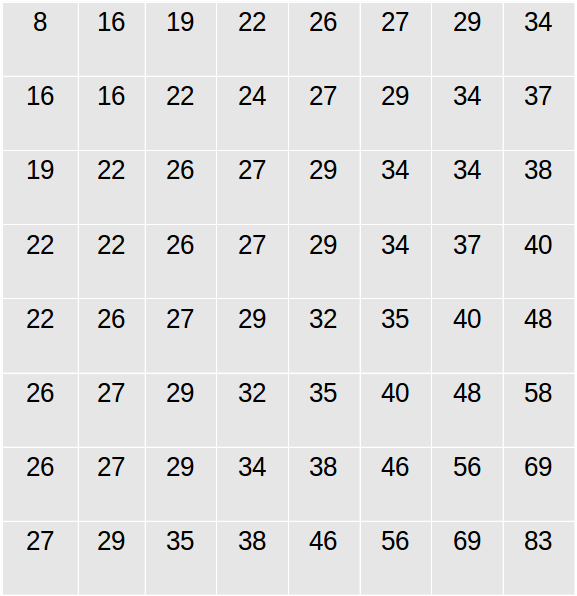
\includegraphics[width=.5\textwidth, height=.5\textwidth]{./Figures/png/tabela_intra.png}}
\subfigure[]{\label{fig:tabela_inter}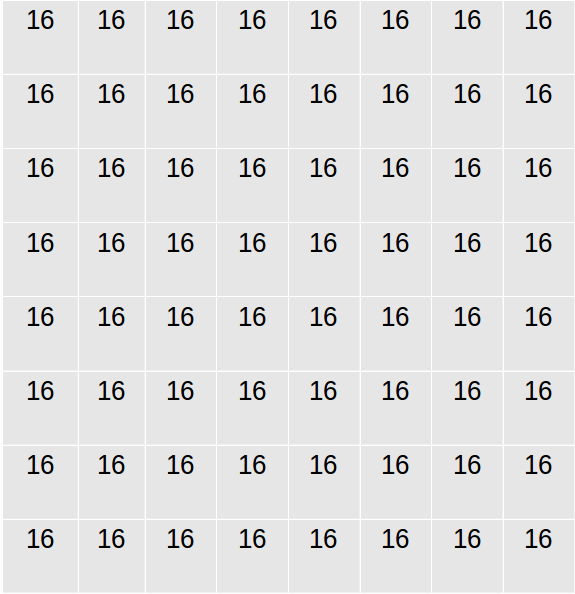
\includegraphics[width=.5\textwidth, height=.5\textwidth]{./Figures/png/tabela_inter.png}}
\caption{Tabelas intra (a) e inter (b).}
\label{tabelas_mpeg}
\end{figure}

%\begin{table}[!ht]
%\begin{minipage}{.5\textwidth}
%\centering
%\begin{tabular}{|c|c|c|c|c|c|c|c|}
%\hline
%8 & 16 & 19 & 22 & 26  & 27  & 29  & 34  \\ \hline
%16 & 16 & 22 & 24 & 27  & 29  & 34  & 37  \\ \hline
%19 & 22 & 26 & 27 & 29 & 34 & 34 & 38 \\ \hline
%22 & 22 & 26 & 27 & 29 & 34  & 37 & 40 \\ \hline
%22 & 26 & 27 & 29 & 32 & 35 & 40 & 48  \\ \hline
%26 & 27 & 29 & 32 & 35 & 40 & 48 & 58 \\ \hline
%26 & 27 & 29 & 34 & 38 & 46 & 56 & 69 \\ \hline
%27 & 29 & 35 & 38 & 46 & 56 & 69 & 83  \\ \hline
%\end{tabular}
%\caption{Tabela intra.}
%\label{standard_table_intra_mpeg}
%\end{minipage} 
%\begin{minipage}{.5\textwidth}
%\centering
%\begin{tabular}{|c|c|c|c|c|c|c|c|}
%\hline
%16 & 16 & 16 & 16 & 16 & 16 & 16 & 16 \\ \hline
%16 & 16 & 16 & 16 & 16 & 16 & 16 & 16 \\ \hline
%16 & 16 & 16 & 16 & 16 & 16 & 16 & 16 \\ \hline
%16 & 16 & 16 & 16 & 16 & 16 & 16 & 16 \\ \hline
%16 & 16 & 16 & 16 & 16 & 16 & 16 & 16 \\ \hline
%16 & 16 & 16 & 16 & 16 & 16 & 16 & 16 \\ \hline
%16 & 16 & 16 & 16 & 16 & 16 & 16 & 16 \\ \hline
%16 & 16 & 16 & 16 & 16 & 16 & 16 & 16 \\ \hline
%\end{tabular}
%\caption{Tabela inter.}
%\label{standard_table_inter_mpeg}  
%\end{minipage}
%\end{table}

É importante deixar claro que a necessidade de duas matrizes de quantização está relacionada com o fato de que, para as imagens preditas, as componentes de alta frequência não são necessariamente frequências espaciais, pois também podem ser provenientes do efeito de blocagem e das limitações o processo de compensação de movimento \cite{ghanbari2003standard}. Portanto, a padronização de uma tabela de quantização ponderada para as imagens inter codificadas seria uma tarefa muito complexa.

\subsubsection{Algoritmo}
\label{mpeg:algoritmo}

O padrão H.261 não reconhece entradas entrelaçadas, por isso utiliza-se a denominação de ``imagens'' e não ``frame''. Há três tipos de imagens que podem ser classificadas em dois métodos de compressão:

\begin{enumerate}
\item Intra imagem: as imagens I, como são conhecidades, são imagens que são codificadas de forma semelhante ao padrão JPEG. Neste tipo de codificação não há redução de redundância temporal, logo exige um volume de dados considerável para armazenamento.

\item Inter imagens: são imagens que passam pelo processo de compensação de movimentos em que as imagens de erro geradas são codificadas de forma semelhante ao JPEG.

Nesta classe se encaixam dois tipos de imagens, imagens P e B, que alcançam diferentes taxas de compressão:

\begin{itemize}
\item P (predita): basicamente a imagem é processada com base na imagem I ou P anterior, em que os vetores de deslocamento partem da imagem anterior para a imagem atual. Estas imagens alcançam maiores taxas de compressão quando comparadas com as imagens I.

\item B (bidirecionalmente predita): imagem processada com base na imagem I anterior e na imagem P posterior, ou vice sersa. A possibilidade de escolha entre dois erros de predição e o erro interpolativo possibilita que estas imagens alcancem taxas maiores de compressão quando comparadas com as imagens P.
\end{itemize}

\end{enumerate}

O processamento de imagens inter codificadas possui maior complexidade quando comparado com as imagens I, não apenas pela compensação de movimento mas também por casos especiais que ocorrem durante o processo de codificação, como:

\begin{enumerate}
\item A anulação de vetores de deslocamento ocorre em situações em que o erro de predição usando um vetor não nulo pode ser muito próximo do obtido através de um vetor nulo, pois neste caso a codificação dos vetores de deslocamento pode gerar a expansão do volume de dados necessários para a representação de um macrobloco.

Este é o procedimento padrão, a não ser que o erro de predição a partir de vetores não nulos seja no mínimo $ 1,1 $ vez menor que o obtido por vetores nulos.

\item Os macroblocos podem ser intra ou inter codificados. Pois há vezes em que a codificação intra é mais vantajosa do que a a inter.

\item Os macroblocos podem ou não ser codificados. A não codificação é utilizada quando todos os coeficientes quantizados da DCT são nulos, neste caso este macrobloco será uma cópia do presente na imagem de referência anterior.
\end{enumerate}

Para o codificador (Fig. \ref{fig:mpeg_enc}), inicialmente os canais Cb e Cr são subamostrados segundo o padrão 4:2:0 e define-se a ordem dos tipos de imagens dentro de um grupo de imagens (GOP, do inglês \textit{group of images}), de acordo com as necessidades. A mais comum é mostrada na figura \ref{fig:image_seq}.

\begin{figure}[!ht]
\begin{center}
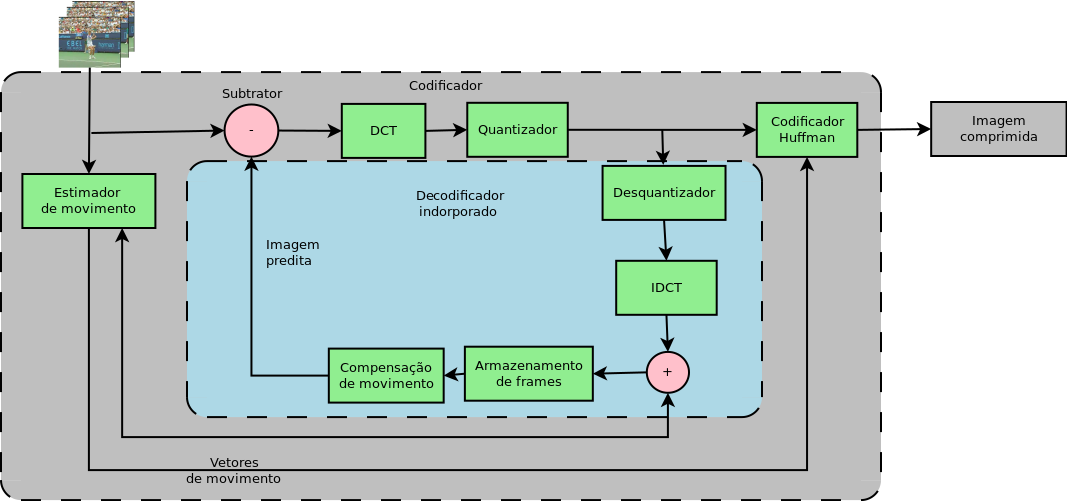
\includegraphics[scale=0.4]{./Figures/png/mpeg_encoder.png}
\caption{Diagrama em blocos do codificador MPEG.}
\label{fig:mpeg_enc}
\end{center}
\end{figure}

\begin{figure}[!ht]
\begin{center}
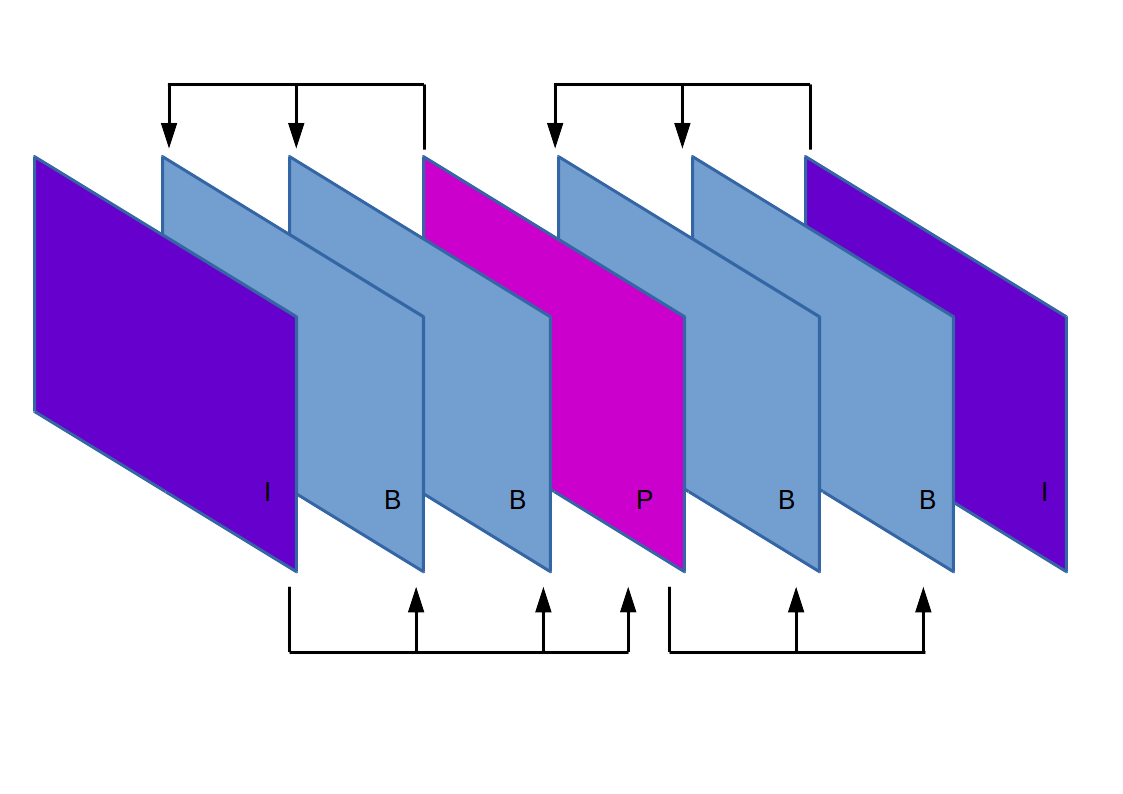
\includegraphics[scale=0.4]{./Figures/png/image_seq.png}
\caption{Sequência de imagens dentro de um GOP.}
\label{fig:image_seq}
\end{center}
\end{figure}

Depois que cada tipo de imagem foi processada, as imagens I, P e B são codificadas conforme descrito no padrão JPEG, porém as duas últimas utilizam a codificação de Huffman descrita no Apêndice \ref{ap_MPEG} para armazenar os vetores de deslocamento.

Para o decodificador (Fig. \ref{fig:mpeg_dec}), deve-se trabalhar por grupos de imagens, recuperando as imagens segundo o decodificador JPEG e recuperando as imagens ($P_1,P_2,P_3,...,P_n$) originais na ordem I, P, B, B, I, B e B para, se for necessário, realizar a compensação de movimento.

\begin{figure}[!ht]
\begin{center}
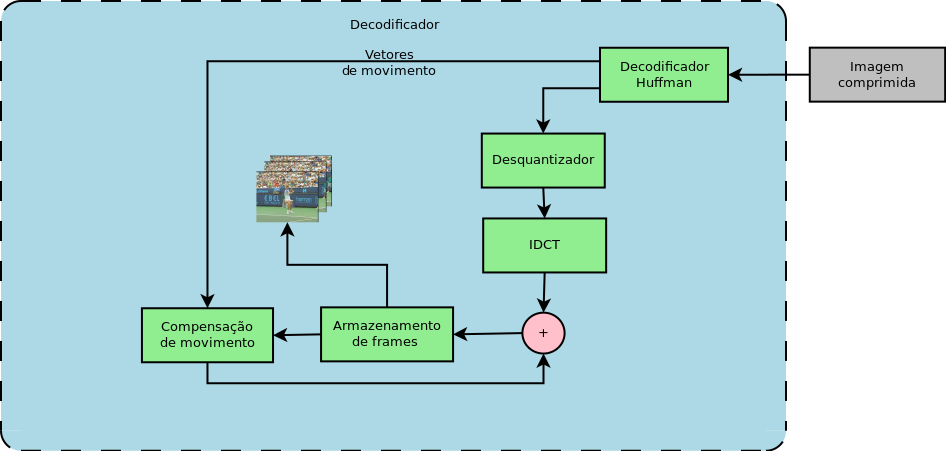
\includegraphics[scale=0.4]{./Figures/png/mpeg_decoder.png}
\caption{Diagrama em blocos do decodificador MPEG.}
\label{fig:mpeg_dec}
\end{center}
\end{figure}